\section{Evaluation}

TODO EVALUATION

The goal of our tool is to help company decision-makers make better decisions with respect to the status quo.
To ascertain the effectiveness of our tool at meeting this goal, we conducted a user study with people in tech to verify that the answers in the treatment group scored better than control with respect to a rubric we created, for a set of dilemmas we selected.
Additionally, we wanted to see if, overall, there was a time difference in the responding between the two groups, and if participants in the treatment group appreciated the tool summary as an aid when answering.

To measure our metrics, we
1) selected the dilemmas
2) recruited people
3) divided into control and treatment, with minutes and pay and task
4) created a rubric
5) scored the answers

\subsection{Dilemma Selection}
scu dataset, mfc classifier
\subsection{Participants Recruitment}
prolific, roles
\subsection{Participant Groups and Tasks}
control, treatment, form format, pay, time, task, questionnaires
\subsection{Evaluation Rubric}
To compare the quality of answers across the Control and Treatment groups, we needed a way to evaluate responses in a consistent and meaningful way. Since moral dilemmas invite complex, subjective reasoning, we could not rely on simple or automatic measures. Instead, we designed an evaluation rubric that breaks down each response into clear dimensions, allowing us to assess specific aspects of reasoning and communication.

We began by reviewing previous research in areas such as argumentation, dialogue systems, ethical reasoning, and decision-making. Based on this review, we identified six dimensions that best reflect the qualities we wanted to measure. Each dimension is supported by existing literature and was selected to match the goals of our study.

\begin{itemize}
\item \textit{Clarity and Structure.} Does the response express its ideas clearly? Is the reasoning easy to follow and well-organized?\\
\hspace*{0.5em}Based on McTear (2005), who highlights the importance of structure and readability in effective communication.

\item \textit{Relevance.} Does the response stay focused on the moral dilemma? Are the points made directly connected to the question?\\
\hspace*{0.5em}Informed by Habernal and Gurevych (2016), who show that content relevance strengthens argument quality.

\item \textit{Persuasiveness.} Is the argument convincing? Does it use logic, appropriate tone, and structure to support its claims?\\
\hspace*{0.5em}Draws from Johnson and Blair (1977), who emphasize the role of logical and well-structured reasoning in persuasion.

\item \textit{Concern for Long-Term Consequences.} Does the response consider future or societal effects of the proposed action?\\
\hspace*{0.5em}Inspired by the Impact Assessment Card (CSCW~'25), which promotes ethical foresight.

\item \textit{Practical Usefulness.} Is the proposed solution realistic? Could it work in practice?\\
\hspace*{0.5em}Based on Bazerman and Moore (2012), who stress the importance of actionable and realistic decision-making.

\item \textit{Awareness of Context.} Does the response take into account the social, cultural, or situational context of the dilemma?\\
\hspace*{0.5em}Also from the Impact Assessment Card (CSCW~'25), which encourages attention to contextual factors in ethical reasoning.
\end{itemize}

Each dimension was defined using a 5-point Likert scale, ranging from 1 (``very low'') to 5 (``very high''). The rubric itself provided the conceptual framework for evaluating responses, while the actual scoring procedure is described in the following section.

\subsection{Scoring the Answers}
Evaluating subjective responses is inherently challenging, especially when the goal is to compare two groups fairly. To ensure our ratings were both unbiased and reliable, we followed a structured scoring process based on the evaluation rubric described above.

We began by generating three identical scoring files---one for each rater. Each file contained an \texttt{AnswerID} and the six rubric dimensions, but no information about whether the response came from the Control or Treatment group. This ensured that all evaluations were blind to condition.

Each rater independently assigned scores using the 5-point Likert scale across all dimensions. Once all ratings were completed, we reattached the group labels to the responses and calculated inter-rater reliability using Fleiss' Kappa for each dimension. We computed agreement scores separately for Control, Treatment, and the full dataset. Our target was to achieve a Kappa score above 0.6 for all dimensions---commonly accepted as the threshold for substantial agreement.

Initial scores fell short of this threshold in some cases. To address this, we held a calibration session where raters discussed discrepancies, reviewed selected responses, and refined their understanding of the rubric. After this reconciliation, we repeated the scoring where needed and achieved the following agreement levels:

\begin{table}[H]
\centering
\caption{Fleiss' Kappa Scores by Dimension and Group}
\resizebox{0.40\textwidth}{!}{%
\begin{tabular}{lccc}
\toprule
\textbf{Dimension} & \textbf{Control} & \textbf{Treatment} & \textbf{Total} \\
\midrule
Clarity & 0.638 & 0.631 & 0.645 \\
Relevance & 0.627 & 0.794 & 0.733 \\
Persuasiveness & 0.696 & 0.625 & 0.681 \\
Concern for Long--Term Consequences & 0.602 & 0.681 & 0.671 \\
Practical Usefulness & 0.595 & 0.709 & 0.683 \\
Awareness of Context & 0.592 & 0.672 & 0.667 \\
\bottomrule
\end{tabular}
}
\label{tab:kappa}
\end{table}

With these agreement levels in place, we computed the average score across raters for each dimension. This resulted in a final dataset with the following structure: \texttt{AnswerID}, \texttt{DilemmaID}, \texttt{Group}, followed by the six rubric scores. This dataset served as the foundation for the subsequent statistical analysis.

\subsection{Results}

\subsubsection{Overview}

The AI-assisted Treatment group consistently outperformed the Control group across all six evaluative dimensions, with effect sizes ranging from medium to large. These findings remained robust after accounting for non-normal data distributions and multiple hypothesis testing.

\subsubsection{Statistical Approach}

Initial normality testing using the Shapiro-Wilk test revealed violations of normality assumptions in at least one group for each dimension. For example, in the \textsc{Clarity} dimension, the \textit{Control} group yielded $W = 0.8817$, $p = 0.0075$ (significant at $\alpha = 0.05$), indicating departure from normality. Similar violations occurred across other dimensions (e.g., \textsc{Relevance} in the Treatment group: $W = 0.8839$, $p = 0.0083$). Given these violations and the ordinal nature of Likert data, non-parametric Mann-Whitney U tests (one-tailed) were conducted to compare median ratings between groups.

\subsubsection{Primary Findings}

All six dimensions showed statistically significant differences favoring the Treatment group:

\begin{itemize}
    \item \textsc{Clarity}: Treatment (Median = 3.333) vs. Control (Median = 3.000), $U = 439.5$, $p = .0063$. The rank-biserial correlation $r = 0.406$ indicates that 40.6\% of all possible pairwise comparisons between groups favor the Treatment group—a medium-to-large effect.
    
    \item \textsc{Relevance}: Treatment (Median = 4.000) vs. Control (Median = 3.000), $U = 496.5$, $p = .0001$, $r = 0.589$. This effect size means 58.9\% of pairwise comparisons favor Treatment—a large effect.
    
    \item \textsc{Persuasiveness}: Treatment (Median = 3.333) vs. Control (Median = 2.333), $U = 514.5$, $p < .0001$, $r = 0.646$. With 64.6\% of comparisons favoring Treatment, this represents a large effect.
    
    \item \textsc{Long-Term Impact}: Treatment (Median = 4.000) vs. Control (Median = 3.000), $U = 548.5$, $p < .0001$, $r = 0.755$. The strongest effect observed, with 75.5\% of pairwise comparisons favoring Treatment.
    
    \item \textsc{Usefulness}: Treatment (Median = 3.667) vs. Control (Median = 2.000), $U = 531.5$, $p < .0001$, $r = 0.701$. Another large effect, with 70.1\% of comparisons favoring Treatment.
    
    \item \textsc{Context}: Treatment (Median = 4.000) vs. Control (Median = 2.667), $U = 551.0$, $p < .0001$, $r = 0.763$. The second-strongest effect, with 76.3\% of comparisons favoring Treatment.
\end{itemize}

The rank-biserial correlation ($r$) is the most appropriate effect size measure for Mann-Whitney U tests, representing the probability that a randomly selected Treatment participant will score higher than a randomly selected Control participant. Values of 0.1, 0.3, and 0.5 correspond approximately to small, medium, and large effects, respectively.

\subsubsection{Robustness Checks}

To ensure reliable conclusions, several validation procedures were conducted:

\textbf{Confidence Intervals:} Non-parametric 95\% bootstrap confidence intervals were computed for median differences. All intervals excluded zero, confirming statistical significance. Representative examples include \textsc{Clarity} $[0.000, 1.333]$, \textsc{Persuasiveness} $[0.333, 2.000]$, and \textsc{Context} $[1.000, 2.000]$.

\textbf{Multiple Comparisons:} Both Bonferroni correction (adjusted $\alpha = 0.0083$) and False Discovery Rate (FDR) correction were applied to control for inflated Type I error rates across six simultaneous tests. All comparisons remained statistically significant under both correction methods.

\subsubsection{Summary}

The Treatment group demonstrated consistent and substantial advantages across all evaluated dimensions. The convergence of multiple analytical approaches—non-parametric testing, effect size quantification, confidence intervals, and multiple comparison corrections—provides strong evidence for the effectiveness of AI assistance in improving response quality.
\begin{figure*}[t]
    \centering
    % First row
    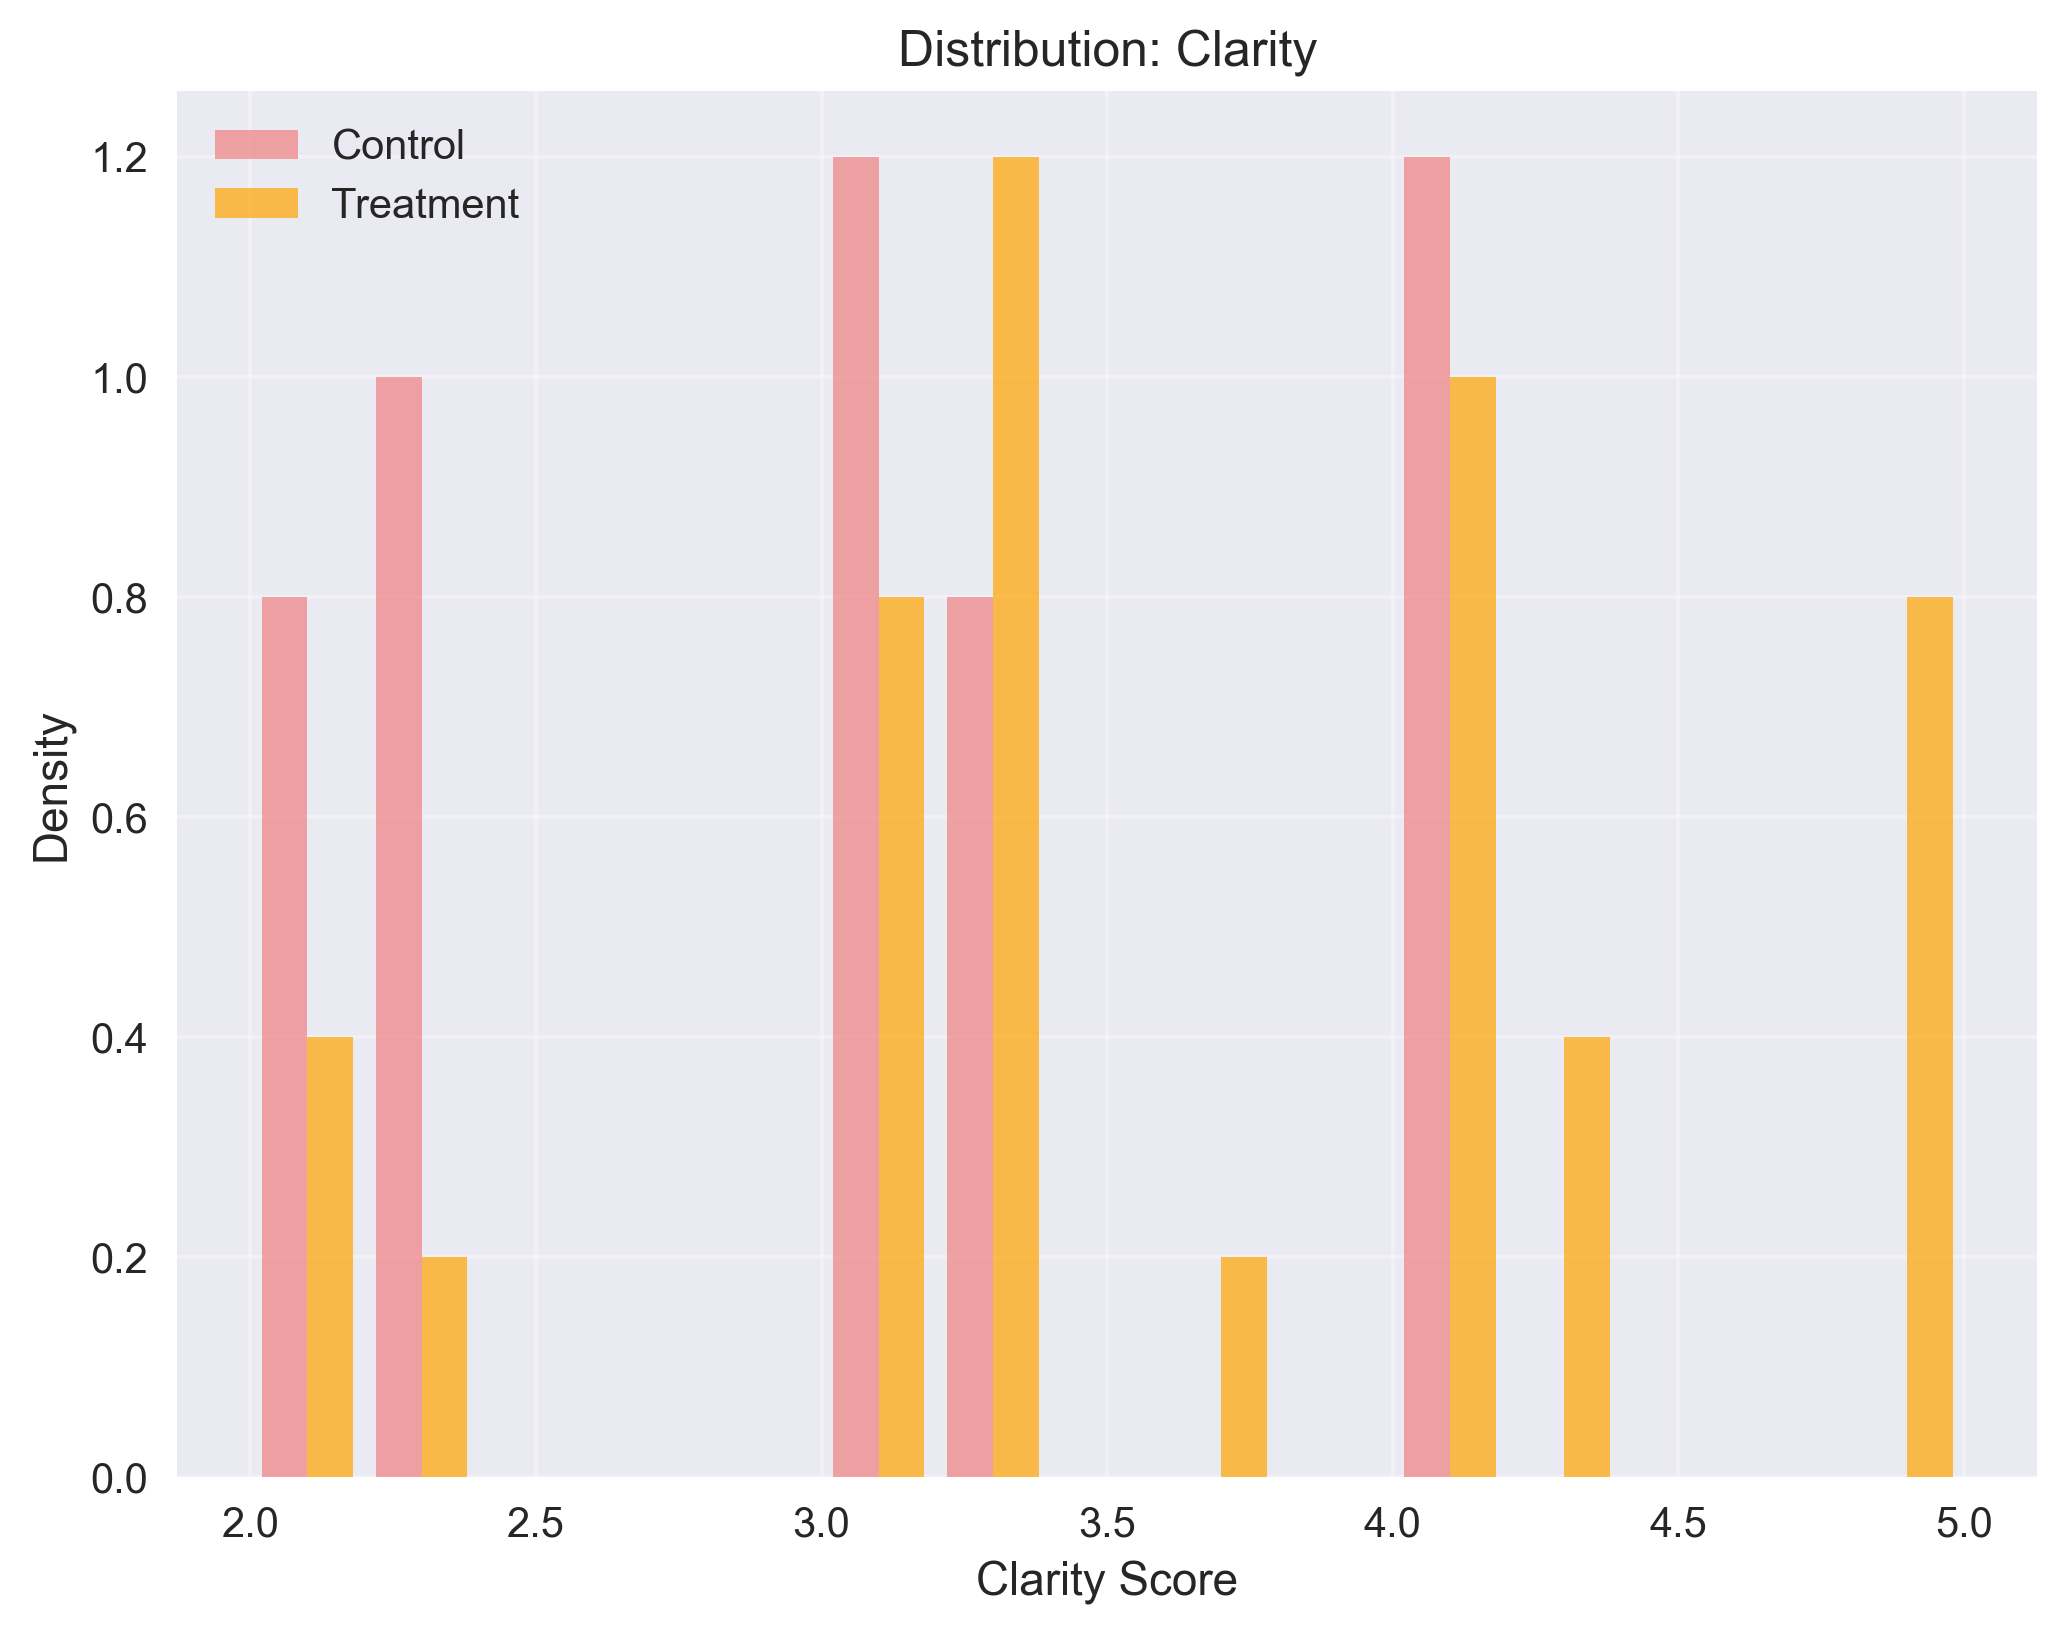
\includegraphics[width=0.3\textwidth]{plots/distribution_clarity.png} \hfill
    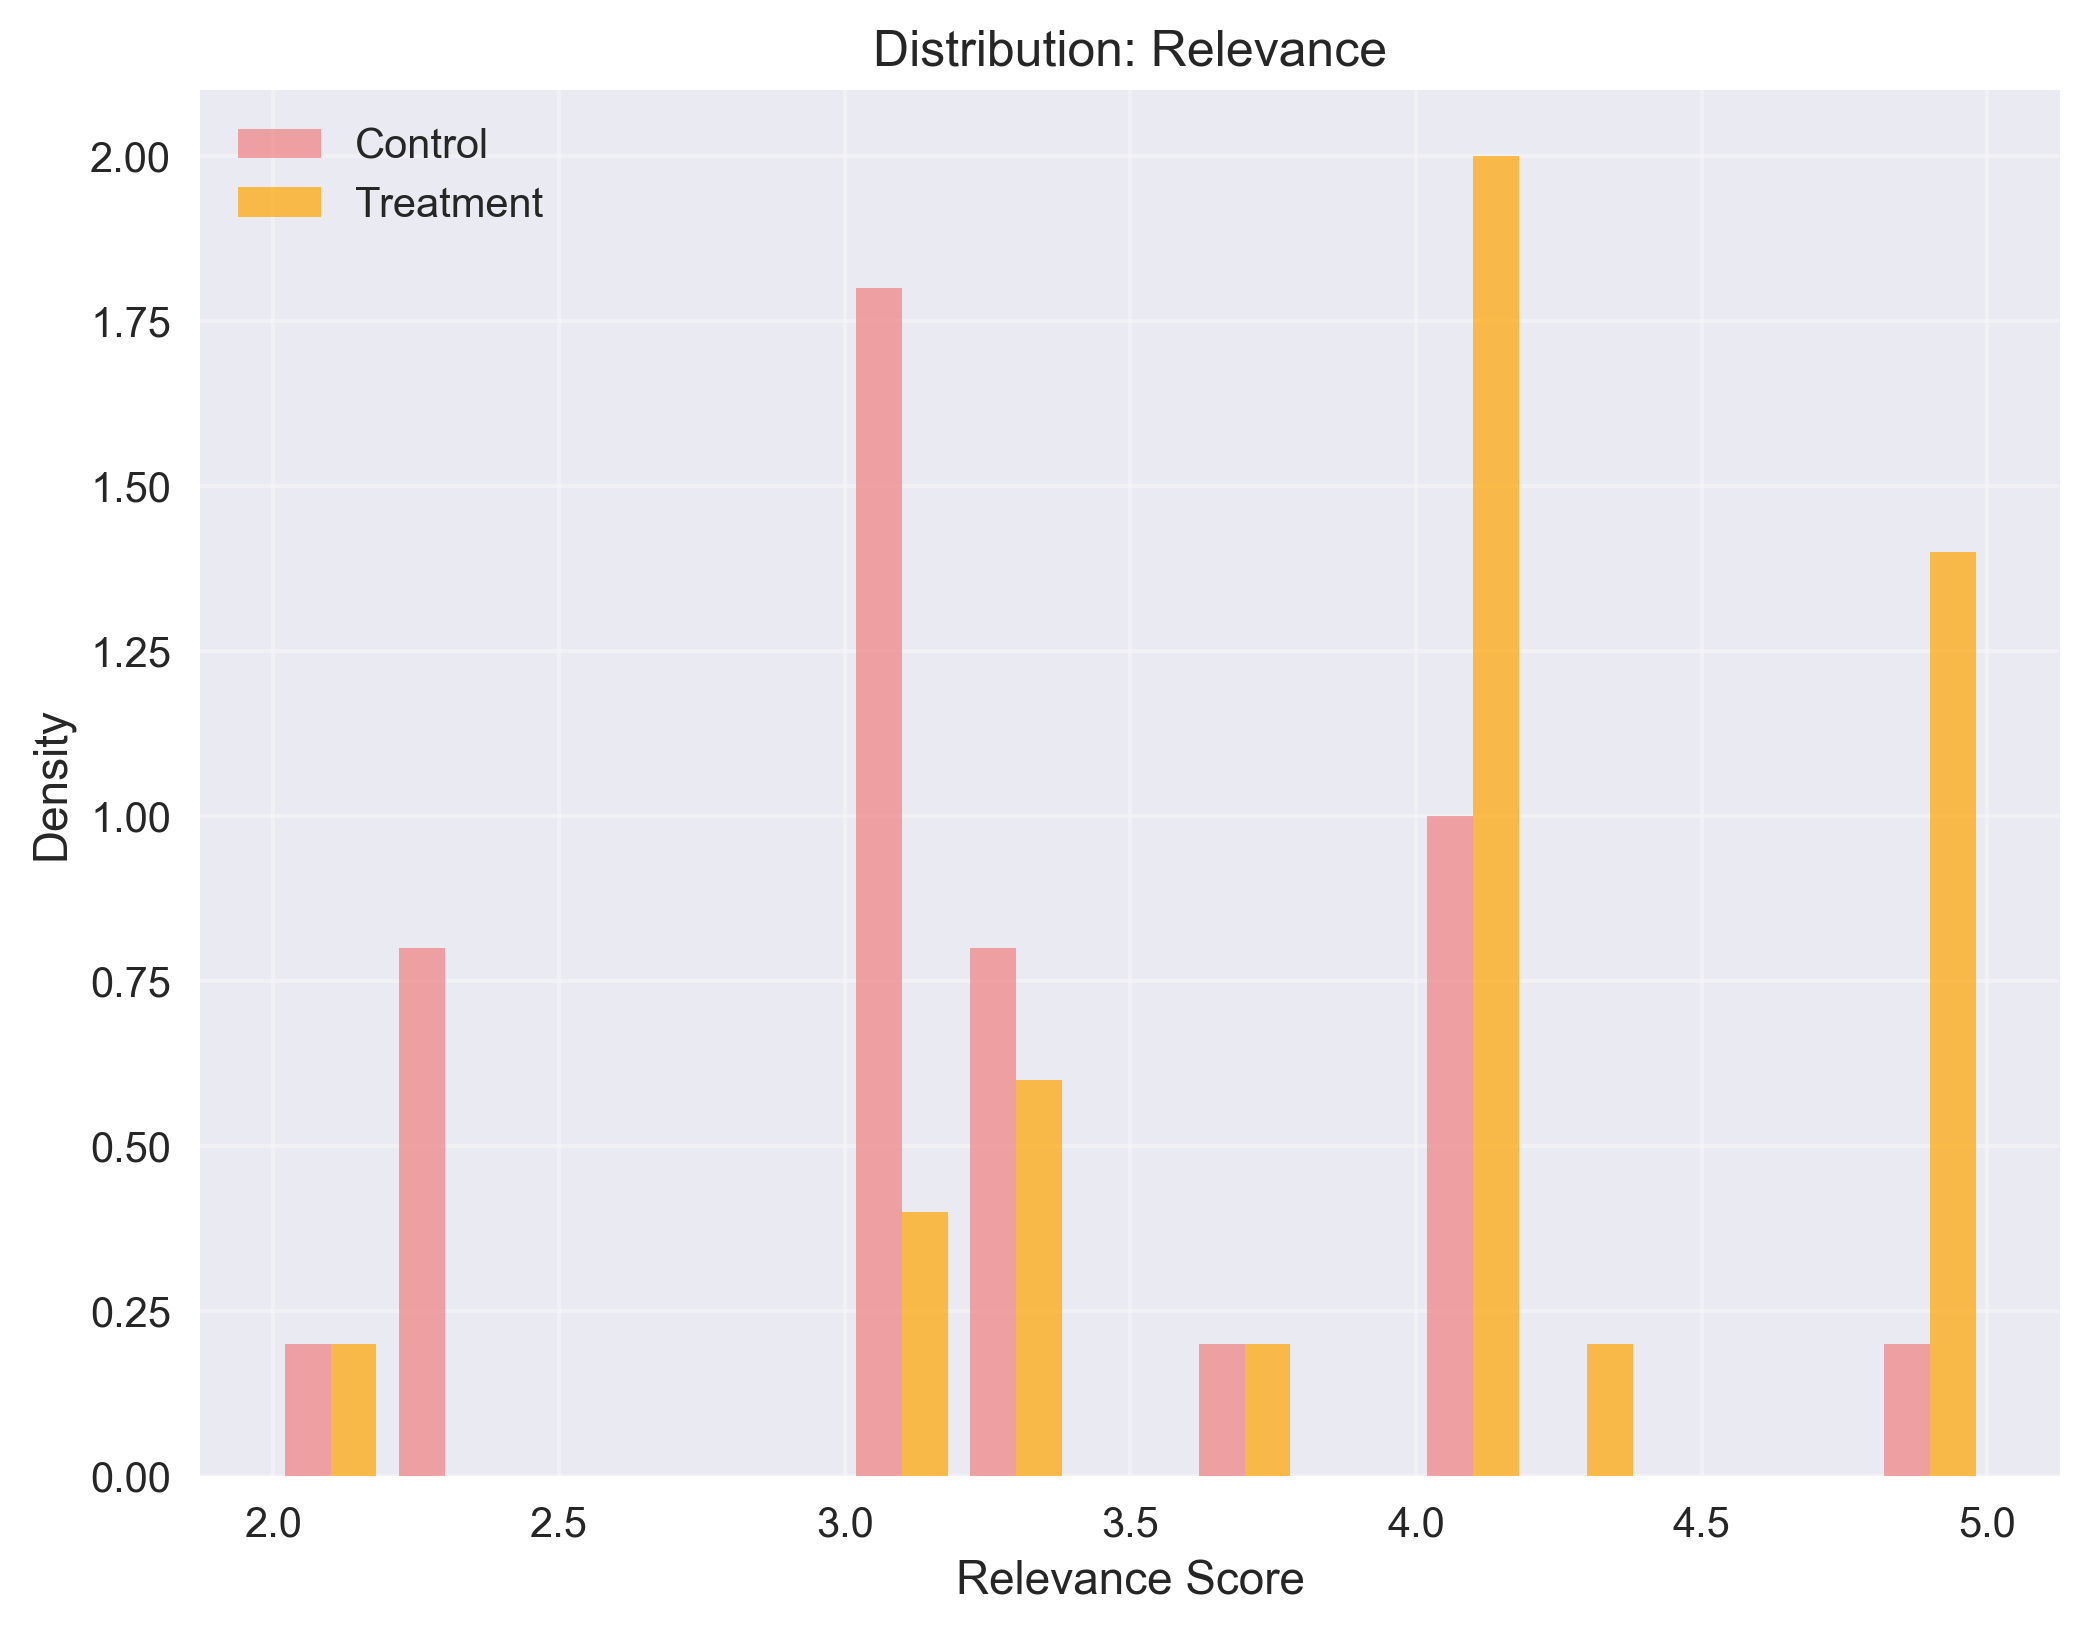
\includegraphics[width=0.3\textwidth]{plots/distribution_relevance.png} \hfill
    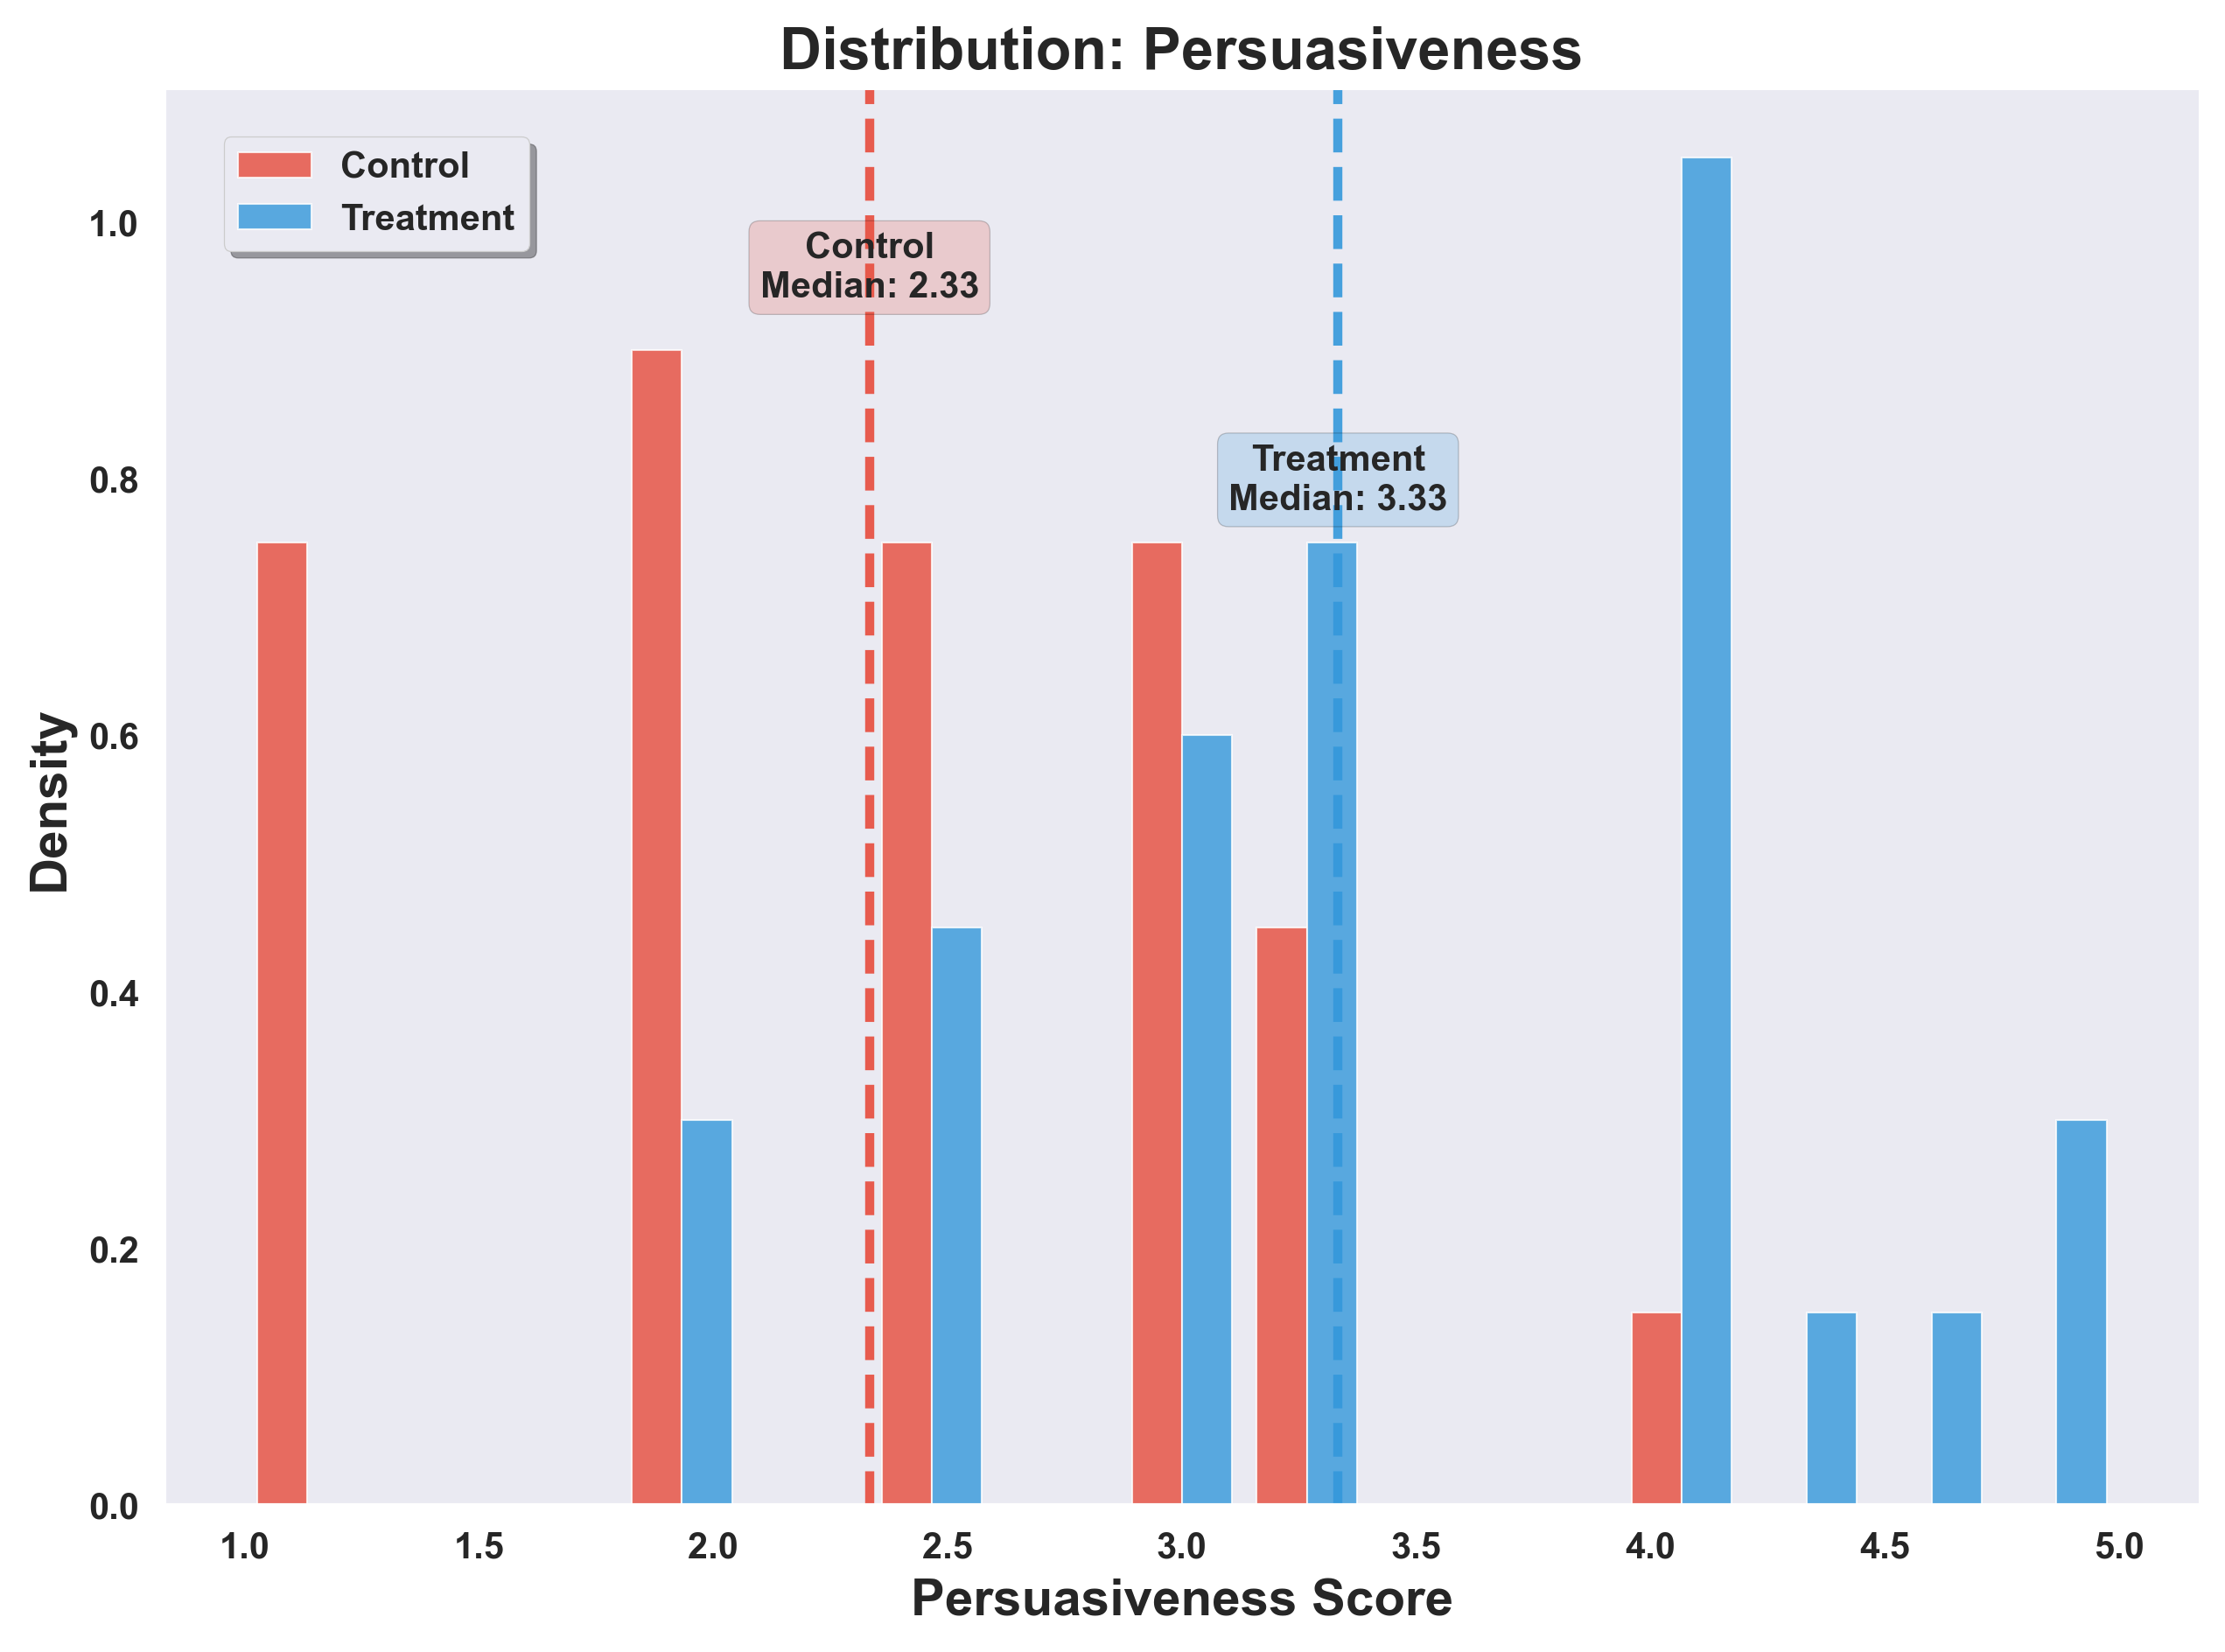
\includegraphics[width=0.3\textwidth]{plots/distribution_persuasiveness.png}
    
    \vspace{1em} % vertical spacing between rows

    % Second row
    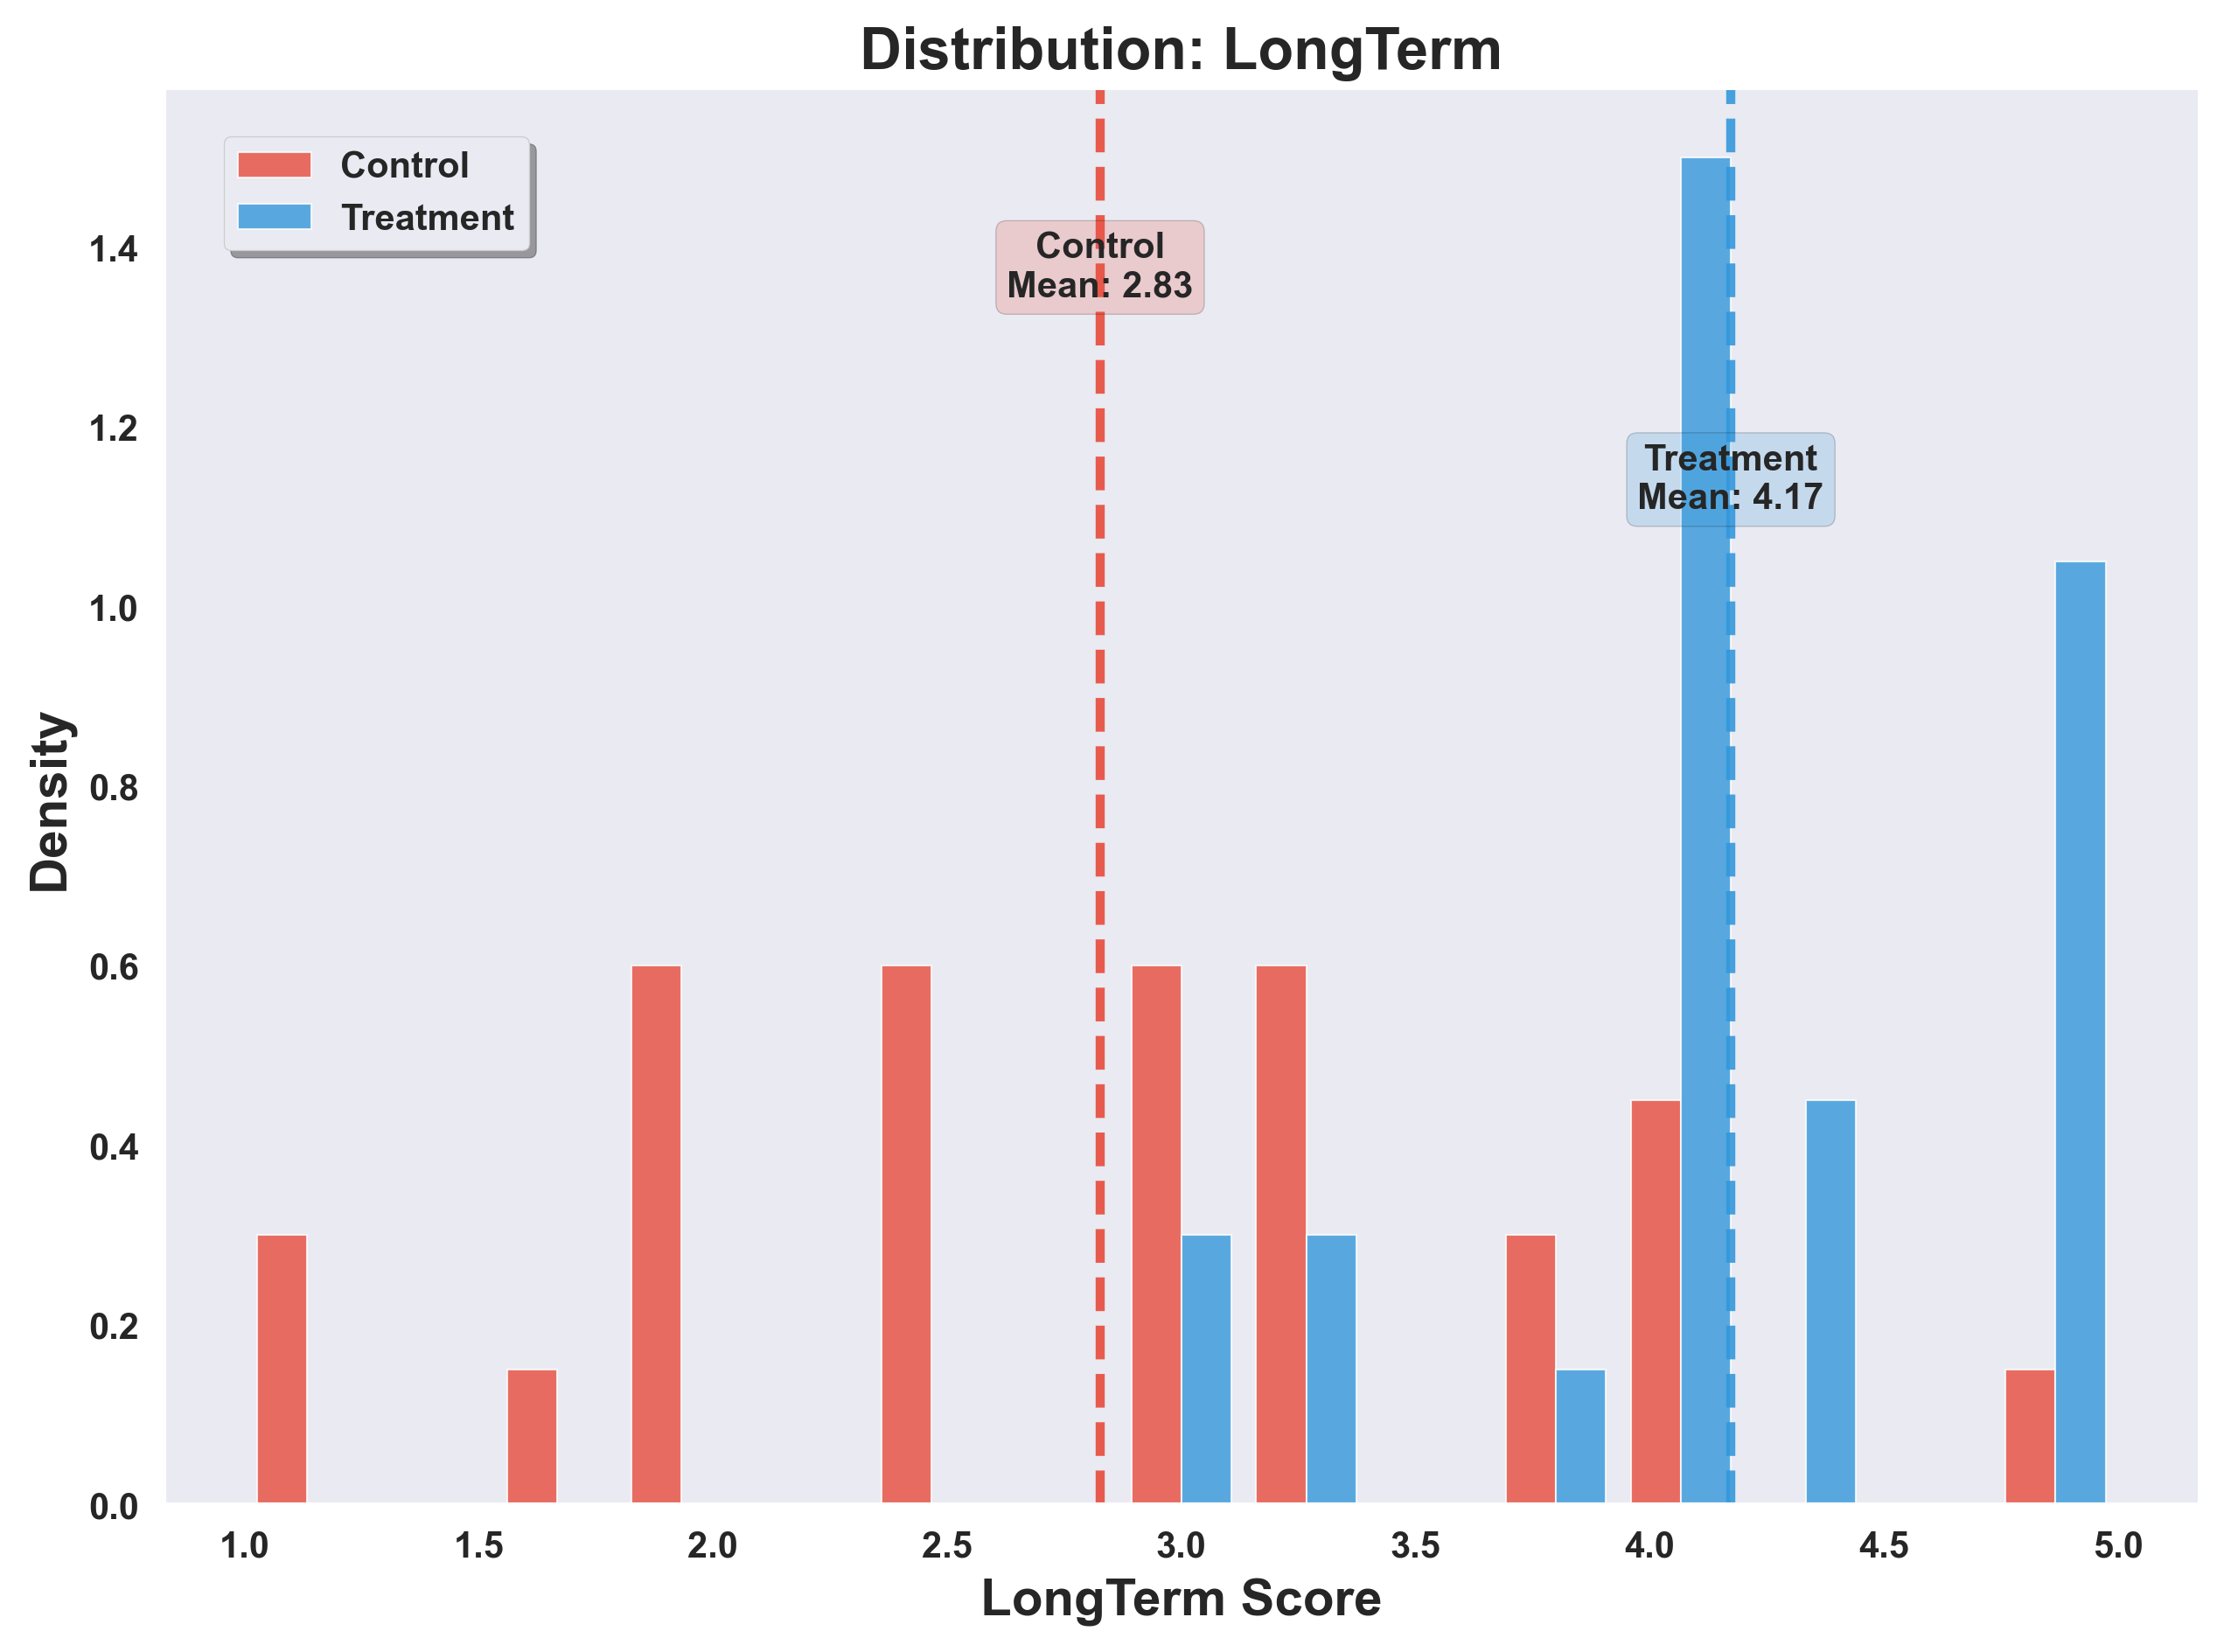
\includegraphics[width=0.3\textwidth]{plots/distribution_longterm.png} \hfill
    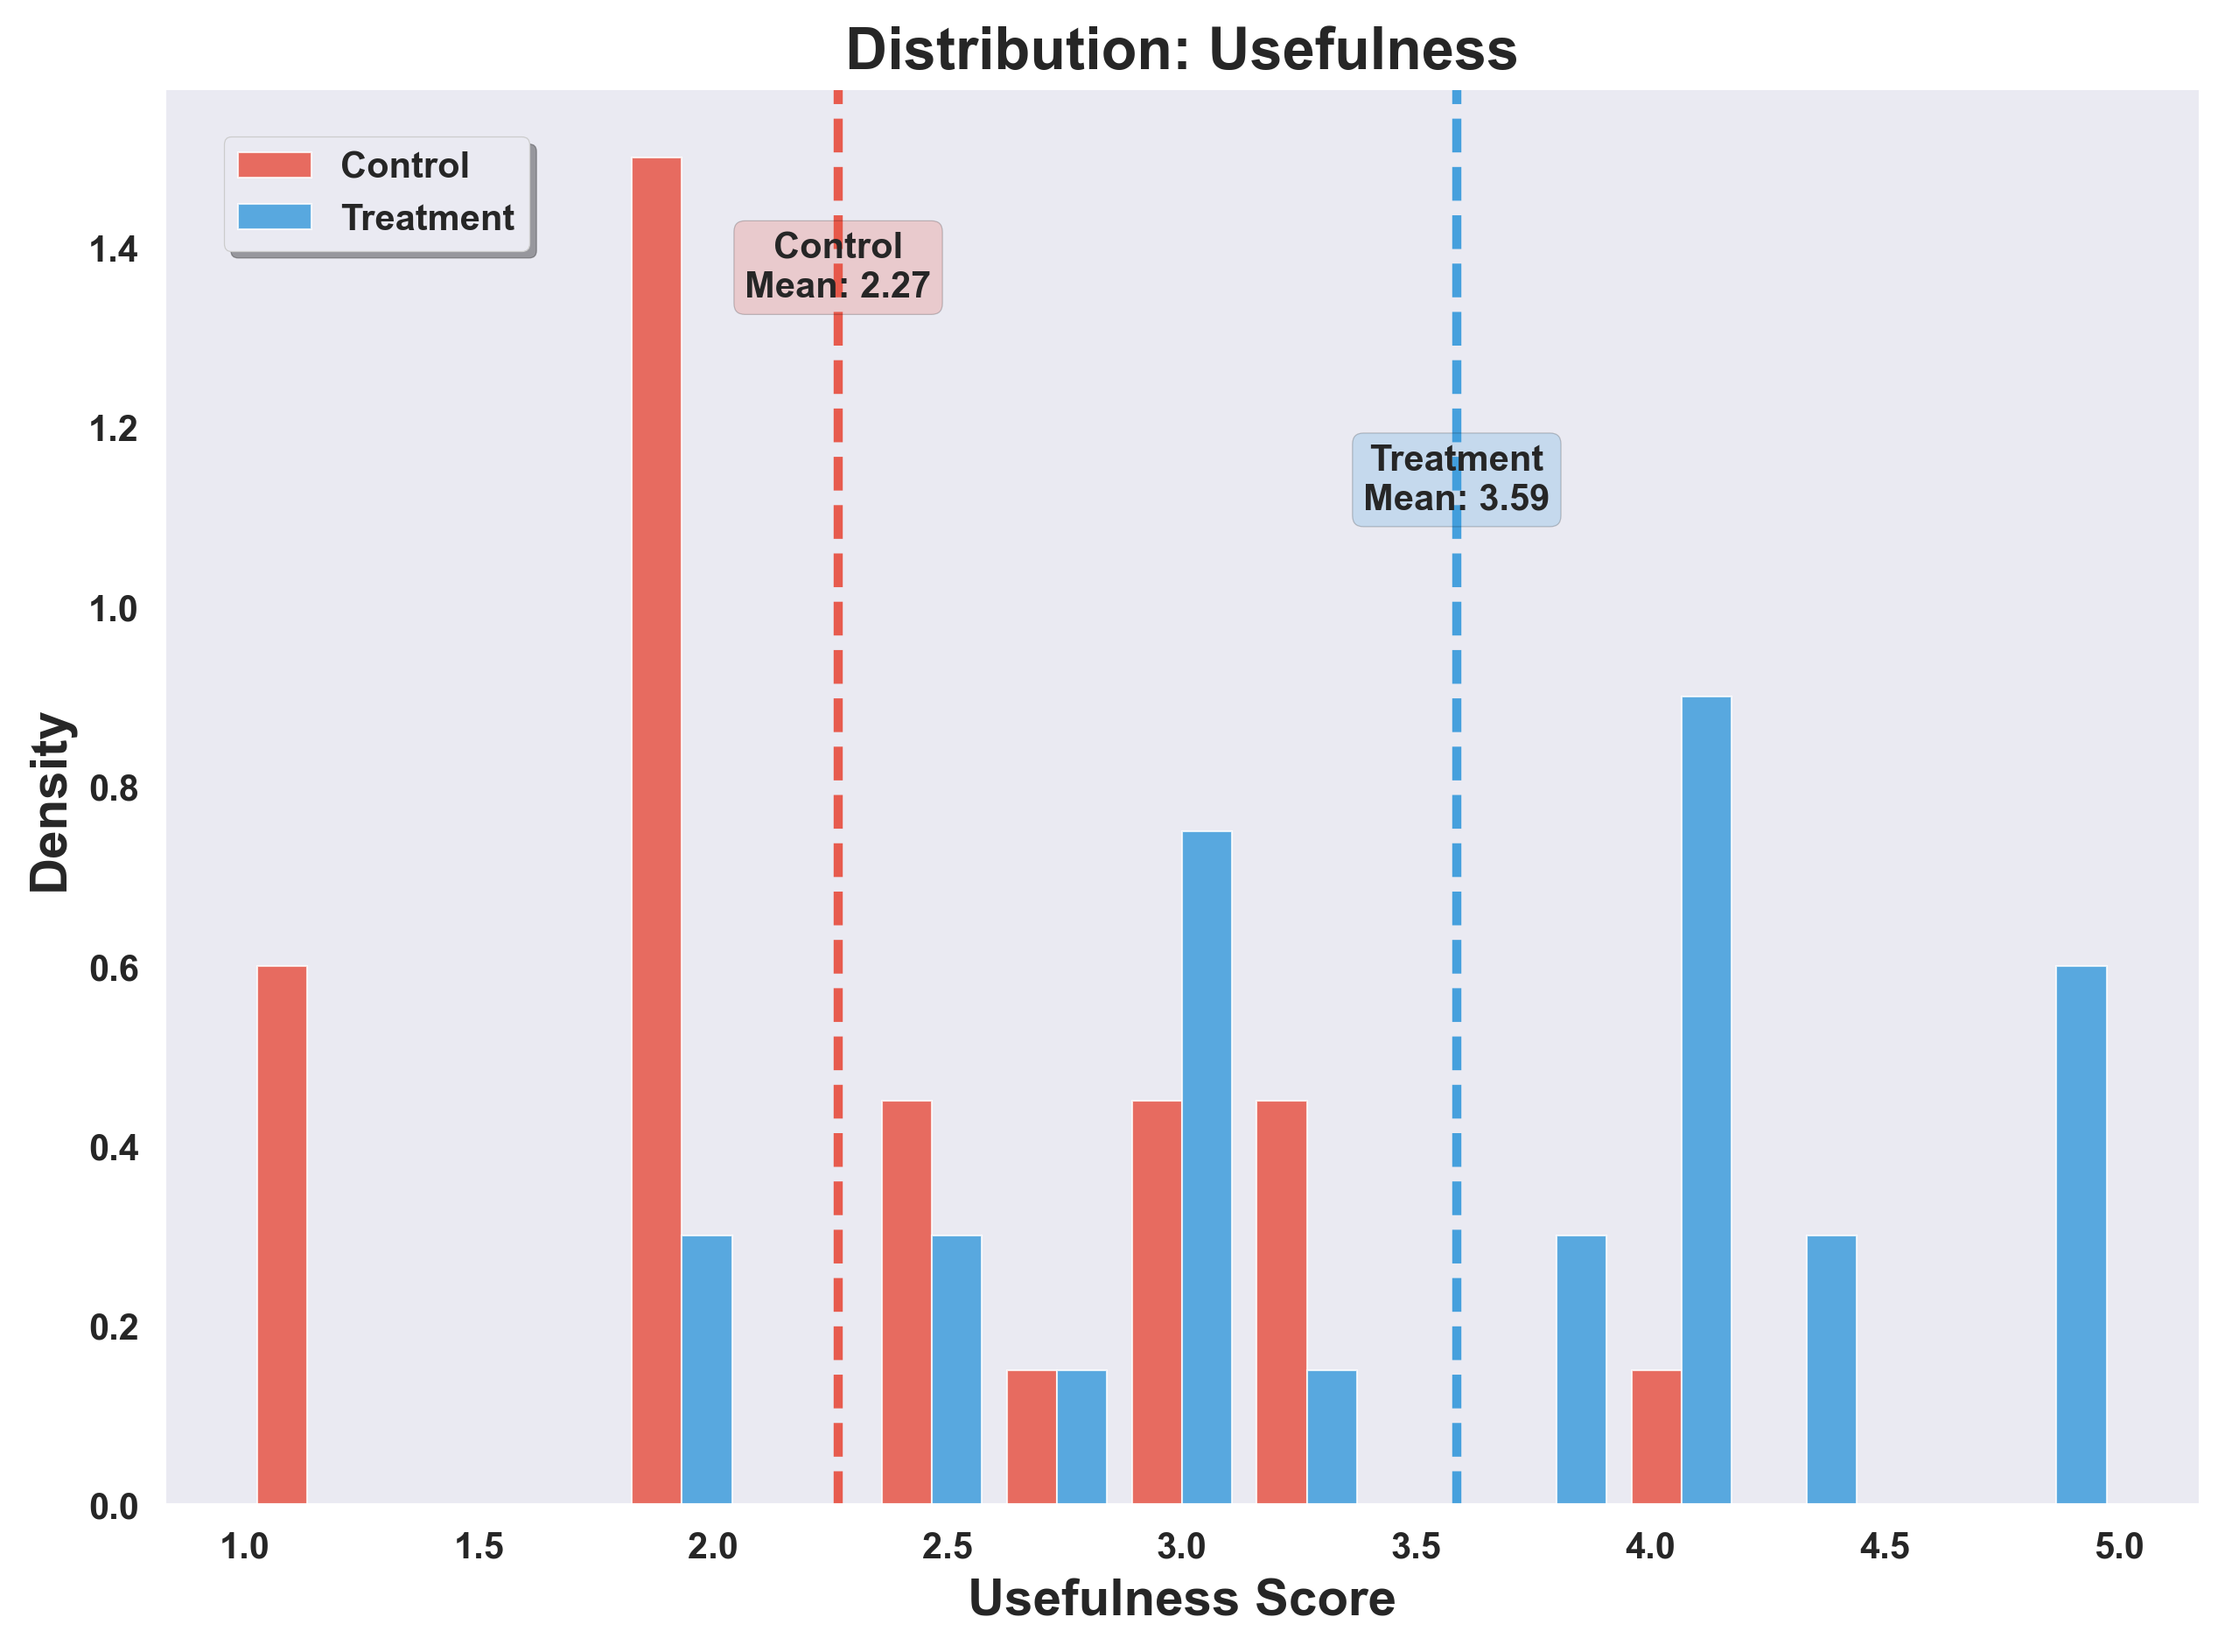
\includegraphics[width=0.3\textwidth]{plots/distribution_usefulness.png} \hfill
    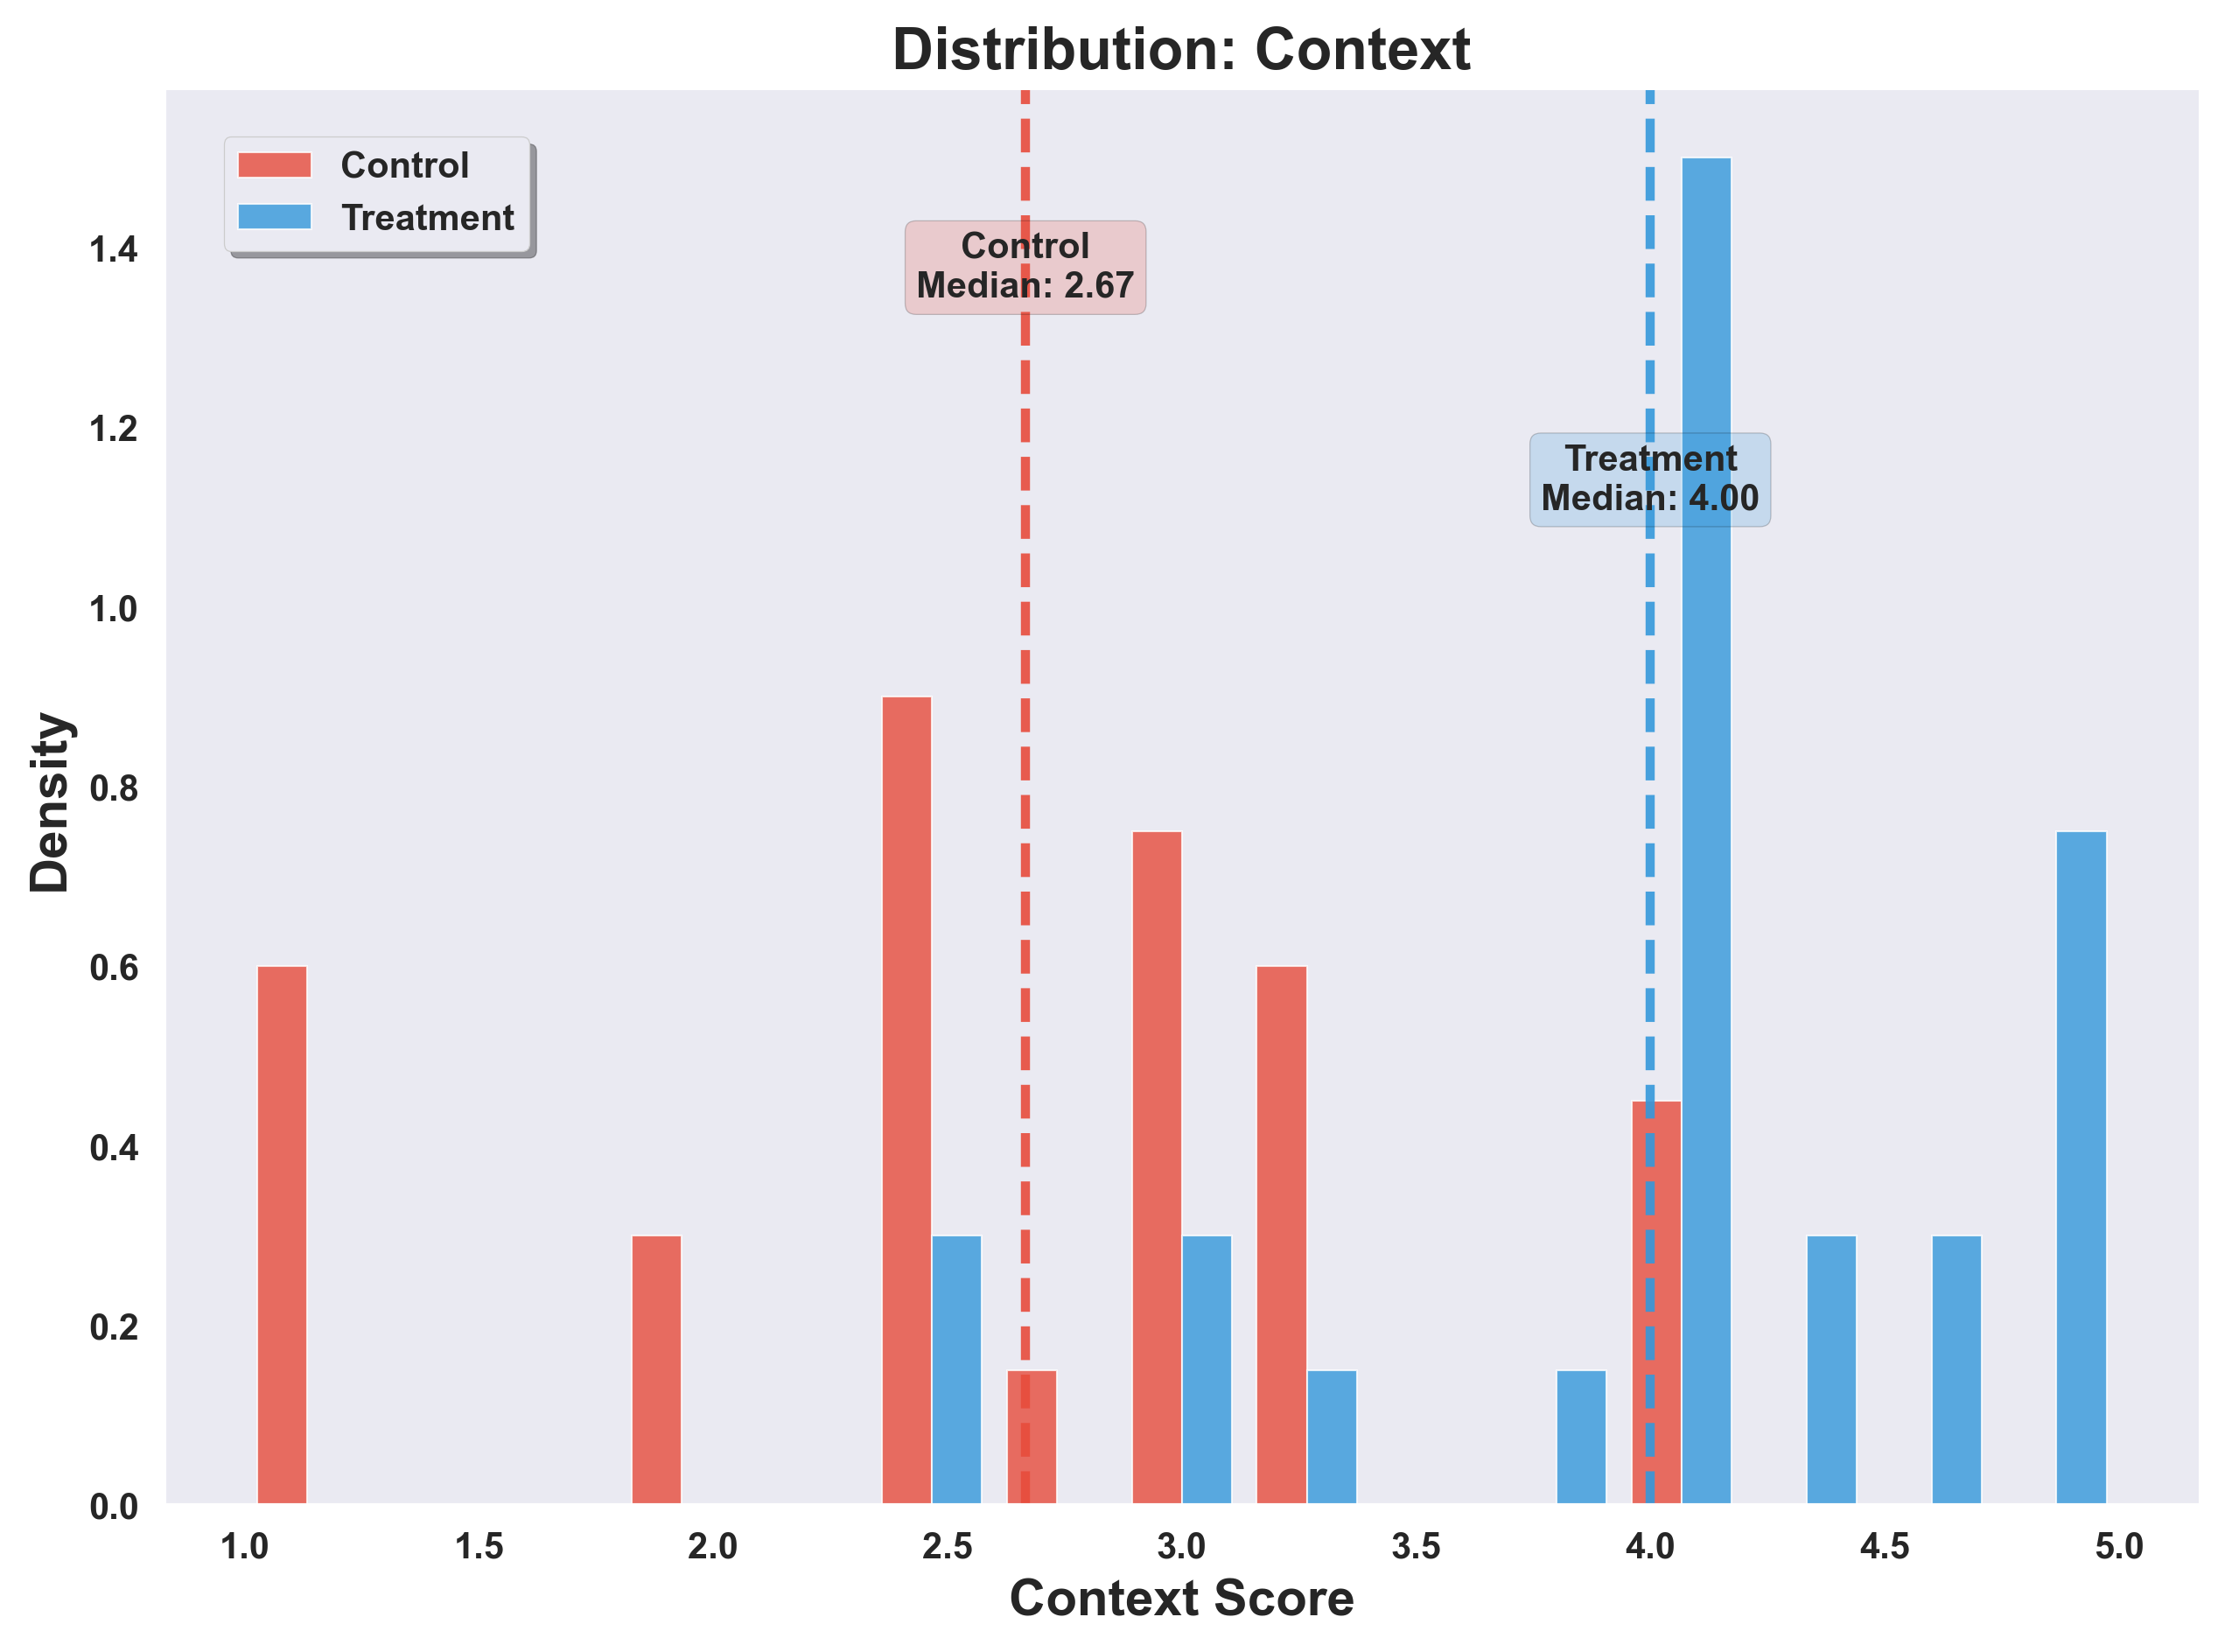
\includegraphics[width=0.3\textwidth]{plots/distribution_context.png}

    \caption{
    Bar plots illustrating distribution of ratings.\\
    Top row: Clarity, Relevance, Persuasiveness (1–3).\\
    Bottom row: Concern for Long--Term Consequences, Practical Usefulness, Awareness of Context (4–6).
    }
    \label{fig:Distribution of Ratings per Dimension}
\end{figure*}

